\section{Overordnet løsningsforslag}

Vi har gennem vores idegenerering kommet frem til to overordnet løsningsforslag. Vi kom frem til at den mest kompliceret dele af kredsen som er vigtigst at designe, og have på plads fra begyndelsen er affyringsmekanismen.
% Mesk kompliceret? Bedre formulering
Heraf har vi kommet frem til to typer afføringsmekanismer: \emph{Gauss-kanon} og \emph{Elastik-kanon}.
Som overordnet løsning til hastighedssensoren har vi tænkt os at se på om vi kan udforme et pass band filter og IR lyd til at sanse hvornår bolden kommer forbi.

\subsection{Gauss-kanon}
Her har vi tænkt os at benytte princippet om magnetfelter i spoler til at drive et projektil fremad. Heraf kan vi ved at variere i den tilførte strømstyrke og spænding for at ændre magnetfeltet.
Ud fra vores brainstorm har vi to måder at udforme sådan en affyringsmekanisme: Magnetisk løb og Magnetisk aftrækker
\subsubsection{Magnetisk løb}
\begin{figure}[H]
	\centering
    \frame{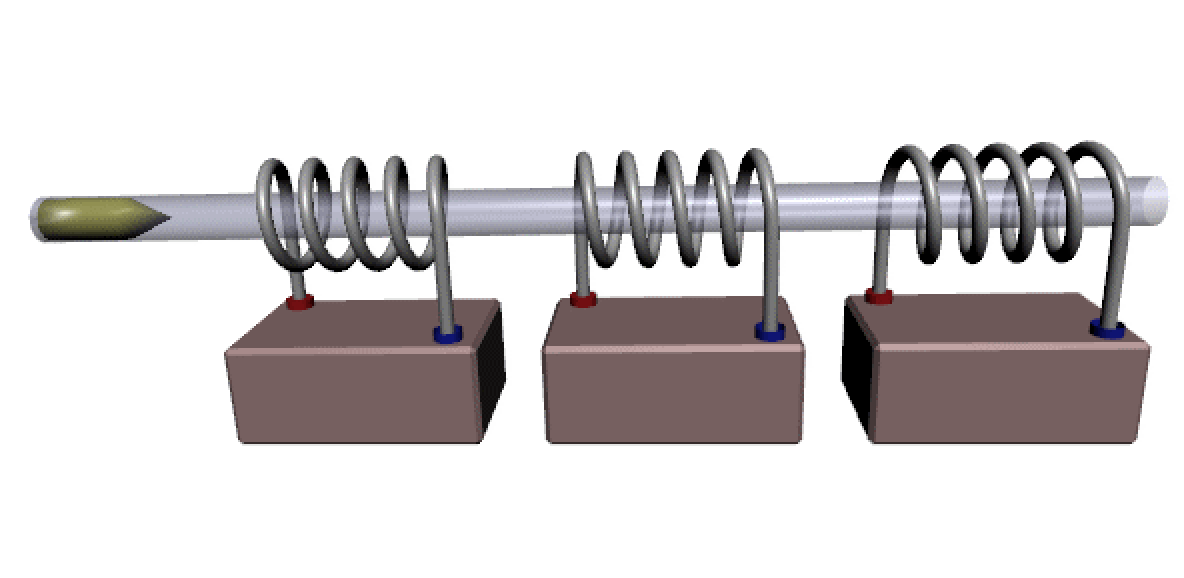
\includegraphics[width=10cm]{figures/2_3overordnetvalg/loeb.png}}
	\caption{Et billede af en gausskanon, hvor projektilet bliver accelereret af tre spoler. Kilde: \cite{WikiGaussCanon}}
	\label{fig:loeb}
\end{figure}
For en enkelt spole, kan et projektils udgangshastighed modelleres udtrykket udformet af PhD i anvendt matematik Don Pettibone (se \cite{gaussRifleModel}).
% Model
\[
	v_{slut} = \frac{\mu_0 \cdot N_0 \cdot I_0}{2 \cdot r_0} \cdot \sqrt{\frac{2 \cdot \mu_r - 1}{\rho \cdot \mu_0}}
\]
\begin{itemize}
	\item $v_{slut}$: Sluthastigheden ved enden af spolen for projektilet $[\frac{\si{m}}{\si{s}}]$
	\item $\mu_0$ : Vakuumpermeabiliteten ($\mu_0 = \SI{1.257d-6}{\frac{T \cdot m}{A}}$).
	\item $I_0$ : Strømstyrke $[A]$.
	\item  $\mu_r$: Relativ permeabilitet af projektilets materiale.
	\item $r_0$: Radius af spolen $\si{[m]}$.
	\item $N_0$: Antallet af vendinger for spolen.
\end{itemize}

Dog er modellen meget optimistisk og i et reelt eksempel (se \cite{HighEffectExample}) udført af elektro-inginøren Mehdi Sadaghdar så vurderer vi at vi kan let komme til at arbejde med effekter på omtrent:
\[
	P \approx \SI{2000}{W}
\]
Måder vi kan holde os fra så store effekter er at benytte jernkerne, for at øge den relative permeabilitet og magneter. Dette er svært at implementere i en Magnetisk løb løsning, idet spoler med jernkerne sjældent har et hul et projektil kan passere. Det er dog lettere at få implementeret i Magnetisk aftrækker løsningen.

En anden måde at få implementeret Magnetisk løb løsningen ved brug af lavere effekter er at benytte et par (knap så lange) solenoider, for at danne en længere spole, således benytte en kombination af sensorer og transistorer til at slukke for den tidligere spole og tænde den næste for at sikre sig at den bliver ved med at accelerer undervejs.

\subsubsection{Magnetisk aftrækker}
Den Magnetiske aftrækker fungerer ved at placerer en magnet tæt ved en slukket spole. Hvis magneten berøre spolens ende der har en tilsvarende ladning vil de afstøde hinanden og således affyre projektet. Se \Cref{fig:MagShooter}.
\begin{figure}[H]
	\centering
    \frame{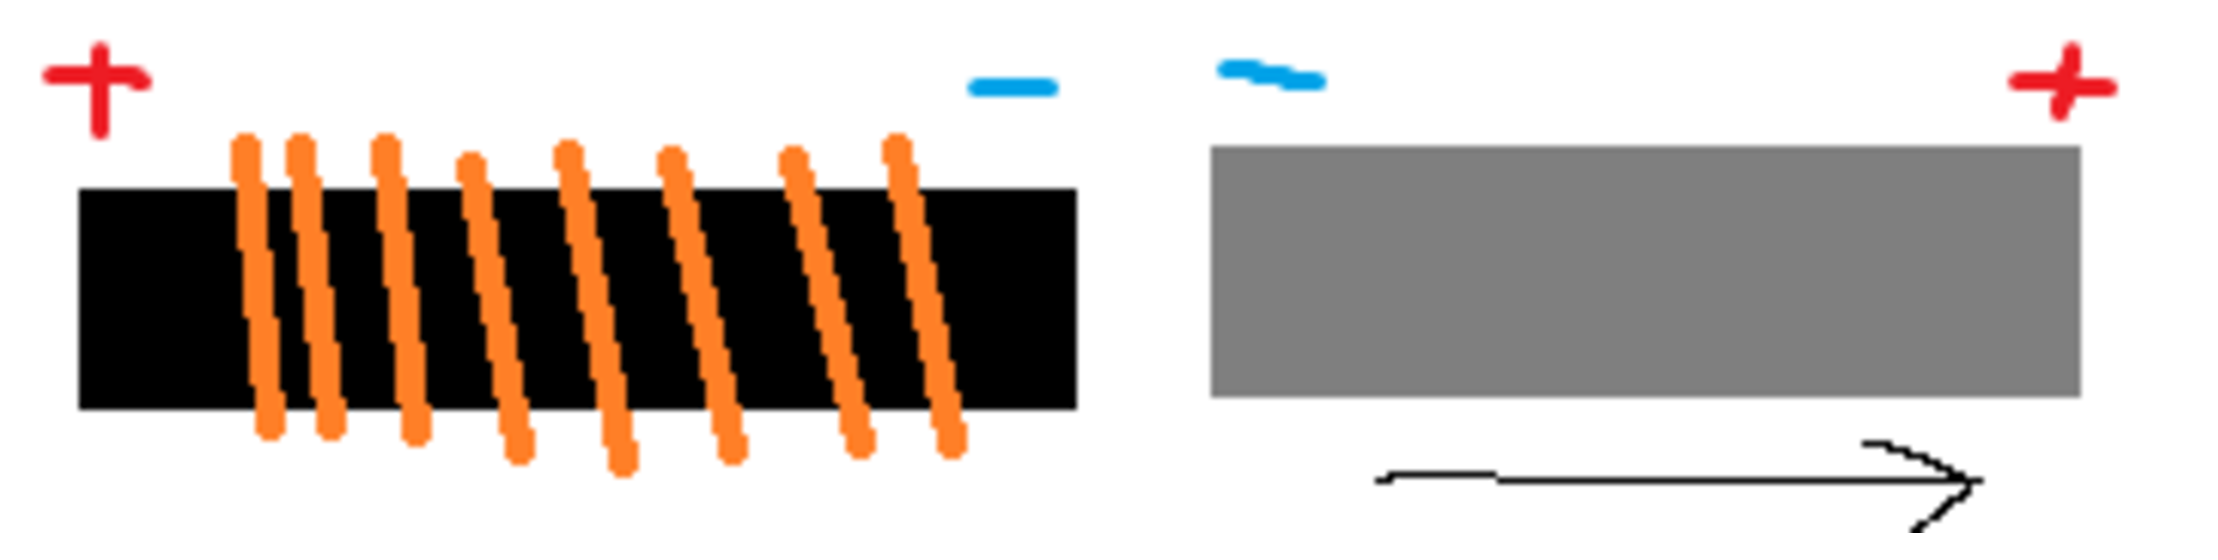
\includegraphics[width=10cm]{figures/2_3overordnetvalg/MagShooter.png}}
	\caption{Et billede af en spole på venstre side, der benyttes til at affyre et magnetisk projektil på højre side.}
	\label{fig:MagShooter}
\end{figure}

Denne løsning er dog svære at matematisk modellere, men med sikkerhed må det gælde at (se \cite{Orbit2009} - side 129), hvis der benyttes jernkerne
\[
	B = \mu_r \cdot \mu_0 \cdot \frac{N_0 \cdot I_0}{l}
\] 
Hvor $B$ er magnetfeltstyrken $[\si{T}]$ og $l$ er længden af spolen $[\si{m}]$. Her fremgår det at hvis $\mu_r$ bliver meget høj (hvilket den kan blive med jernkerne), vil magnetfeltet stige proportionalt. Med passende legeringer kan man få en relativ permeabilitet på op til \num{15000}.


Ulempen ved denne løsning er dog at der nok skal være ret så høj en effekt der skal sendes gennem spolen indenfor et kort tidsrum for at få det til at virke.

\subsection{Elastik-kanon}
Denne løsning bliver vores produkt udformet som en slangebøsse med variabel styrke. Således bliver den variable: hvor langt væk elastikken trækkes væk fra hviletilstand.
En model for dette princip kan simpel konstrueres ud fra energiomdannelse fra potentiel energi i Hooks lov til kinetisk energi.
\begin{align}
-k \cdot x &=\frac{1}{2} \cdot m \cdot v^2 \\
 \iff v	&= \sqrt{\frac{-2 \cdot k \cdot x}{m}} 
\end{align}
\begin{itemize}
	\item $k$: Fjederkonstanten for benyttet elastik $\si{[\frac{N}{m}]}$
	\item $m$: Massen af projektilet $\si{[kg]}$
	\item $v$: Udgangshastigheden af projektilet $\si{[\frac{m}{s}]}$
	\item $x$: Afstand fra hviletilstand $\si{[m]}$
\end{itemize}

Vores implementering af en elastik-baseret løsning er at vi benytter os af en snor der er forbundet til elastikken og et hjul, hvor hjulet drejes af en motor (se \Cref{fig:elasticshooter}). For at sikre os at projektilet bliver affyret benytter vi gear, så når optrækning-mekanisme trækker snoren er hjulet i gear, hvorimod når vi skal affyre projektilet sættes den i frigear. Dette kan gøres ved at lade en motor være den der trækker snoren op, og en anden motor være den der ændrer gear.
\begin{figure}[H] 
	\centering
    \frame{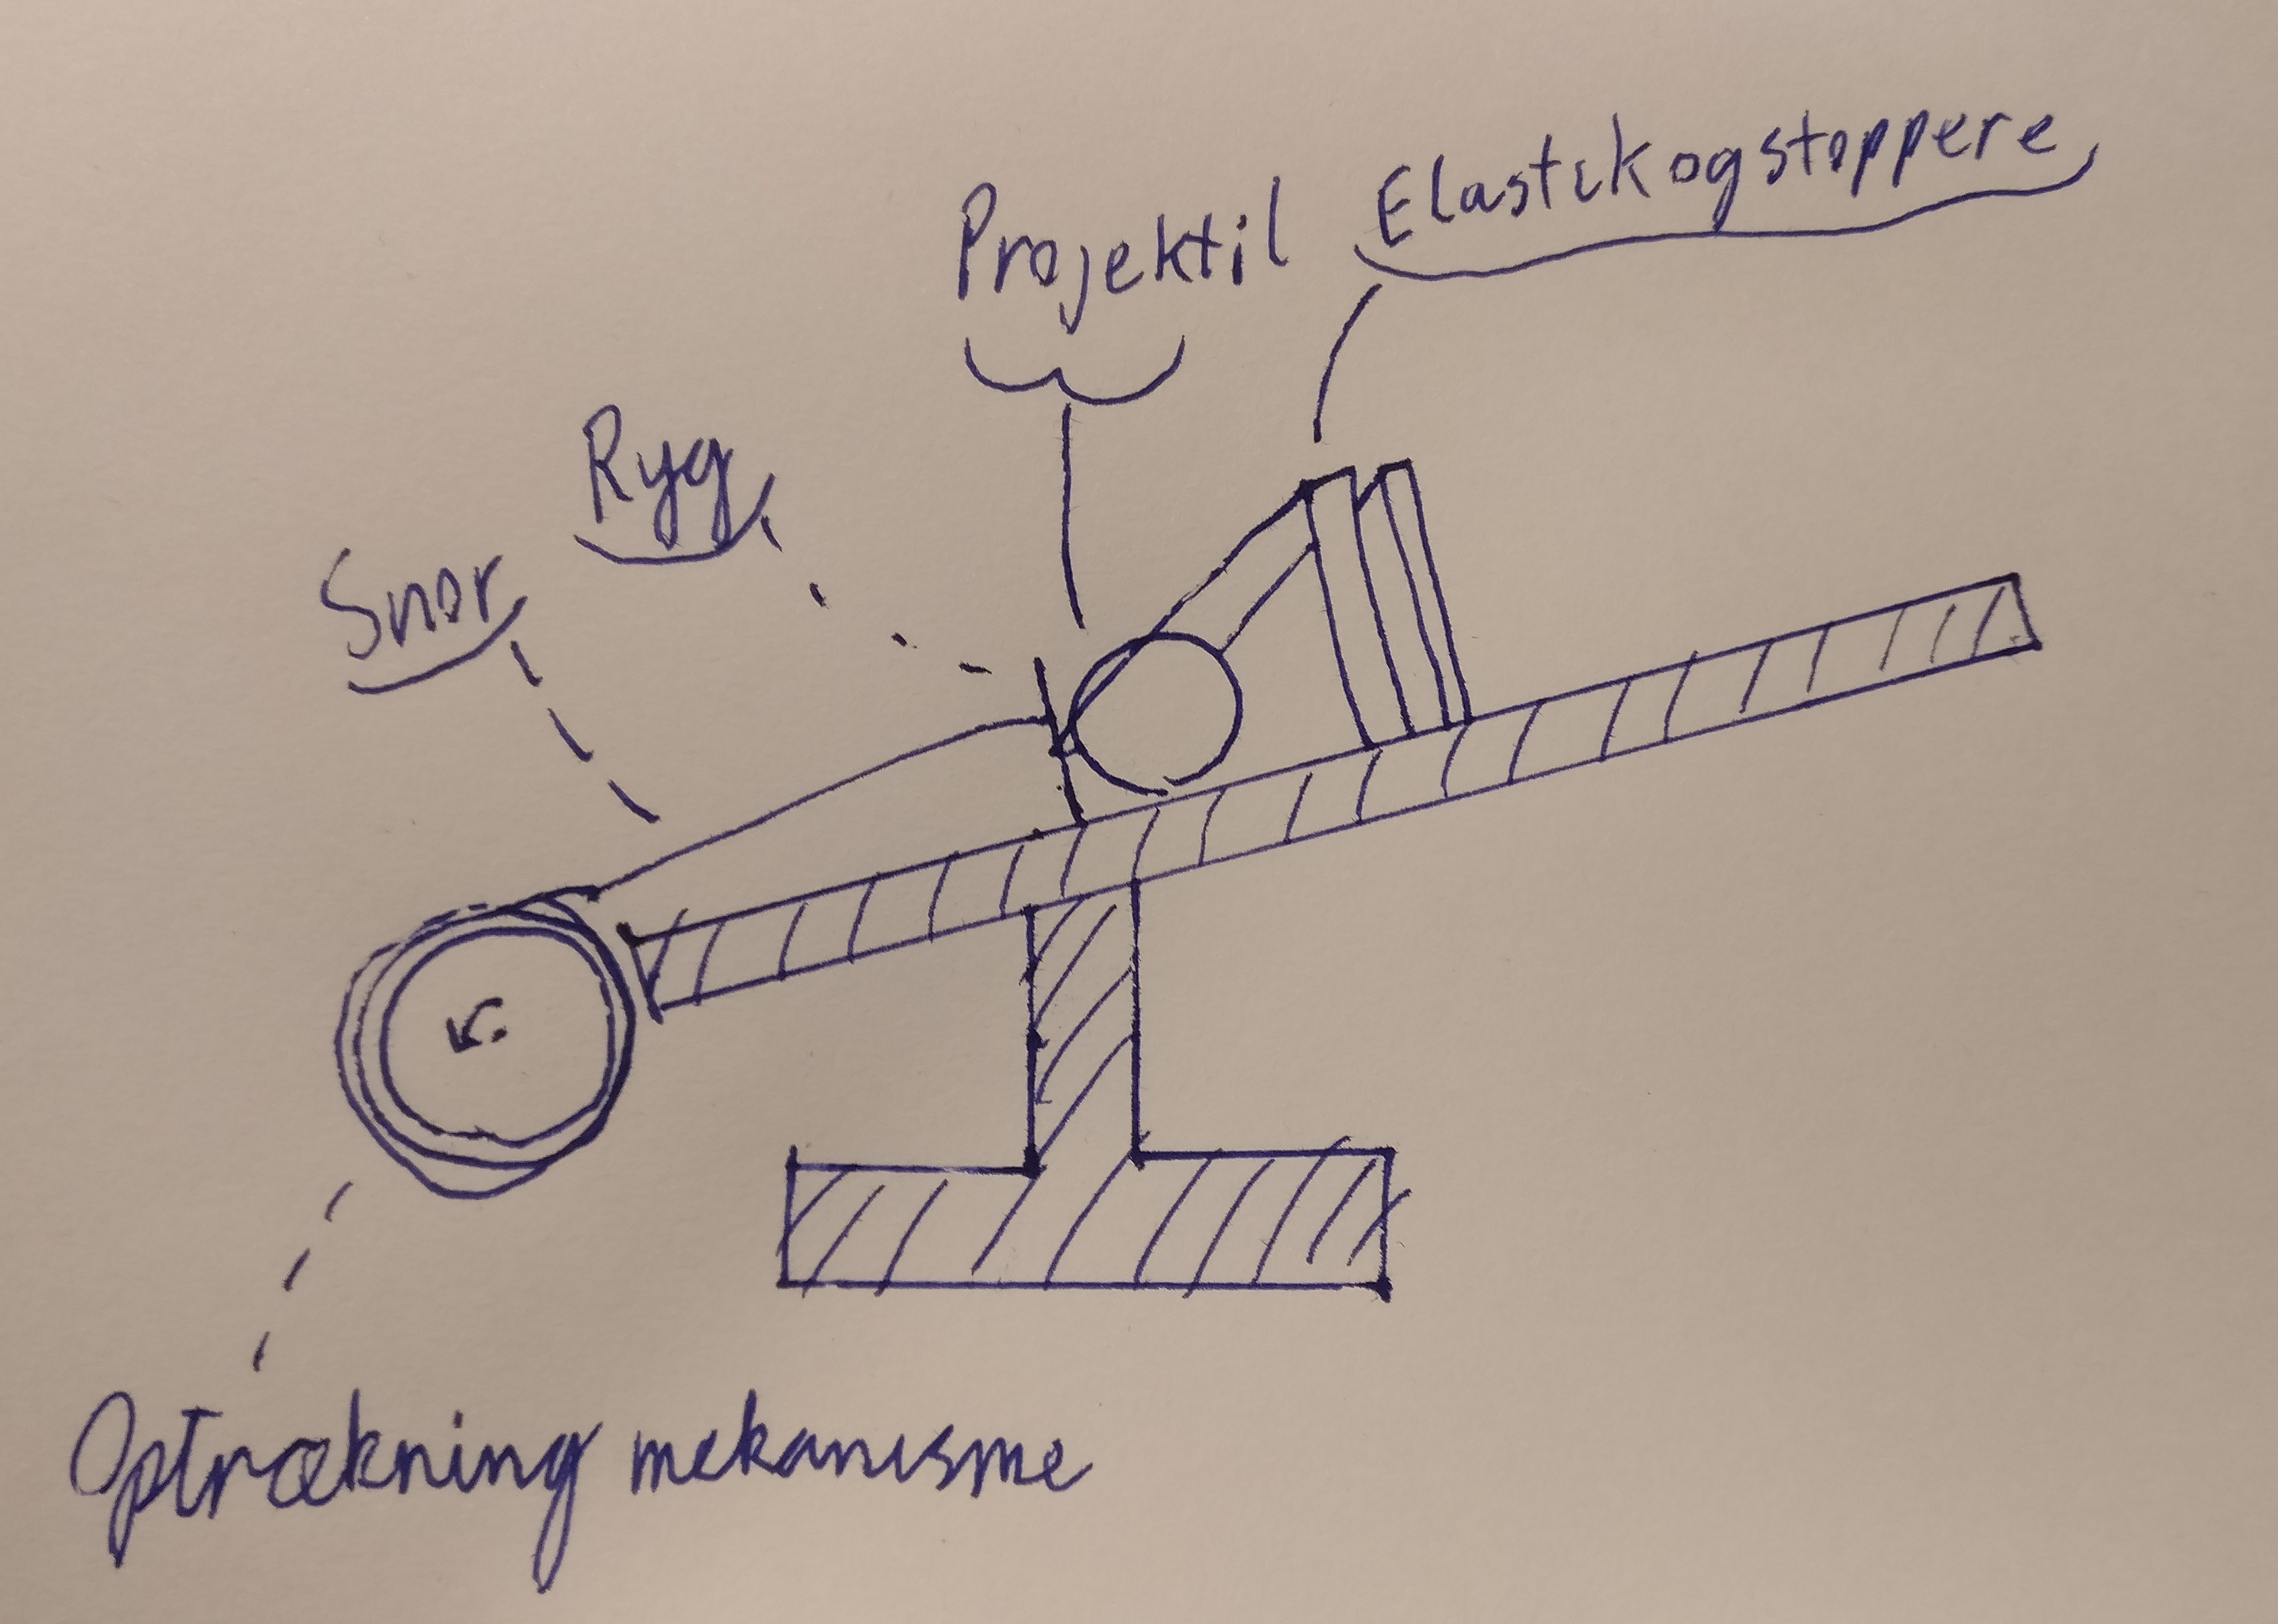
\includegraphics[width=13cm]{figures/2_3overordnetvalg/ElasticShooter.jpg}}
	\caption{Affyringsmekanisme for en Elastik-kanon, der er ikke fokus på andre blokke beskrevet i projektbeskrivelse.}
	\label{fig:elasticshooter}
\end{figure}


\subsection{Valg af overordnet løsning}
Vi har valgt at udarbejde en Elastik-kanon, idet vi synes hvor får en del EL-problemer at se til i forhold til hastighedssensoren. Samt hvis vi skulle udarbejde en Gauss-kanon, ville vi bruge lang tid på at teste for vakuumpermeabilitet og benytte høje strømstyrker, hvilket i sig selv kunne give en del problemer, da vi ikke ved meget om at arbejde med høje strømstyrker. Samt ville man kunne argumentere for at så høje strømstyrker som benyttes i forbindelse med en Gauss-kanon kan muligvis være for farligt til et børnelejetøj.

